\documentclass[11pt]{article}

\usepackage{fancybox}



\usepackage{color}
\usepackage{url}
\usepackage[margin=1in]{geometry}


\renewcommand{\textfraction}{0.0}
\renewcommand{\topfraction}{1.0}
%\renewcommand{\textfloatsep}{5mm}




\usepackage{comment}
% Definitions of handy macros can go here
\usepackage{amsmath,amssymb,amsthm,bm,mathtools}
%\usepackage{dsfont,multirow,hyperref,setspace,natbib,enumerate}
\usepackage{dsfont,multirow,hyperref,setspace,enumerate}
\hypersetup{colorlinks,linkcolor={blue},citecolor={blue},urlcolor={red}} 
\usepackage{algpseudocode,algorithm}
\algnewcommand\algorithmicinput{\textbf{Input:}}
\algnewcommand\algorithmicoutput{\textbf{Output:}}
\algnewcommand\INPUT{\item[\algorithmicinput]}
\algnewcommand\OUTPUT{\item[\algorithmicoutput]}

\mathtoolsset{showonlyrefs=true}



\theoremstyle{plain}
\newtheorem{thm}{Theorem}[section]
\newtheorem{lem}{Lemma}
\newtheorem{prop}{Proposition}
\newtheorem{pro}{Property}
\newtheorem{assumption}{Assumption}

\theoremstyle{definition}
\newtheorem{defn}{Definition}
\newtheorem{cor}{Corollary}
\newtheorem{example}{Example}
\newtheorem{rmk}{Remark}


\def\MLET{\hat \Theta_{\text{MLE}}}
\newcommand{\cmt}[1]{{\leavevmode\color{red}{#1}}}



\usepackage{dsfont}

\usepackage{multirow}

\DeclareMathOperator*{\minimize}{minimize}



\usepackage{mathtools}
\mathtoolsset{showonlyrefs}
\newcommand*{\KeepStyleUnderBrace}[1]{%f
  \mathop{%
    \mathchoice
    {\underbrace{\displaystyle#1}}%
    {\underbrace{\textstyle#1}}%
    {\underbrace{\scriptstyle#1}}%
    {\underbrace{\scriptscriptstyle#1}}%
  }\limits
}
\usepackage{xr}
\externaldocument{tensor_regression}
\input macros.tex





\title{Supplements for ``Generalized tensor regression with covariates on multiple modes''}


%\author{%
%Yuchen Zeng \\
%University of Wisconsin -- Madison\\
 %\texttt{yzeng58@wisc.edu} \\
%\And
%Miaoyan Wang \\
%University of Wisconsin -- Madison\\
%\texttt{miaoyan.wang@wisc.edu} \\
%}

\begin{document}


\begin{center}
\begin{spacing}{1.5}
\textbf{\Large Supplements for ``Generalized tensor-response model with multi-sided covariates''}
\end{spacing}
\end{center}

\section{Proofs}
\begin{thm}
Consider a generalized tensor regression model with multi-sided covariates $\tX=\{\mX_1,\ldots,\mX_K\}$. Suppose the entries in $\tY$ are independent realizations of an exponential family distribution, and $\mathbb{E}(\tY|\tX)$ follows the low-rank tensor regression model~\eqref{eq:tensormodel}. Under Assumption~\ref{ass}, there exist two absolute constants $C_1, C_2>0$, such that, with probability at least $1-\exp(-C_1\sum_k p_k)$, 
\begin{equation}\label{eq:bound}
\text{Loss}(\trueB,\ \hat \tB) \leq C_3\sum_k p_k,
\end{equation}
where $C_3=C_3(\mr)={1\over C^{2K}_2U}{\prod_k r_k \over \max_k r_k}>0$ is a constant that does not depend on the dimensions $\{d_k\}$ and $\{p_k\}$. 
\end{thm}


\begin{proof}[Proof of Theorem 1]

Let $\ell(\tB)=\mathbb{E}(\tL_{\tY}(\tB))$, where the expectation is take with respect to $\tY\sim \trueB$ under the true parameter. We show that 
\begin{enumerate}
\item[C1.] The stochastic deviation $\tL_{\tY}(\tB)-\ell(\tB)$ is uniformly small for all $\tB\in\tP$,
\item[C2.] There exist two positive constants $c_1, c_2>0$ such that 
\[
c_1 \FnormSize{}{\hat \tB-\trueB}^2 \leq \ell(\hat \tB) - \ell(\trueB) \leq  c_2\FnormSize{}{\hat \tB-\trueB}^2.
\]
\end{enumerate}

To prove C1, note that 
\begin{align}
\tL_{\tY}(\tB)-\ell(\tB)&=\langle \tY-\mathbb{E}(\tY|\tX),\ \Theta(\tB)\rangle\\
&= \langle \tY- b'(\trueT),\ \Theta\rangle \\
&= \langle \tE\times_1\mX^T_1\times_2\cdots\times_K\mX^T_K,\ \tB\rangle,
\end{align}
where $\tE=\entry{\varepsilon_{i_1,\ldots,i_K}}\stackrel{\text{def}}{=}\tY-b'(\trueT)$. Based on Assumption A1, $\tE$ is a sub-Gaussian tensor with parameter bounded by $C_1=\phi U$. Therefore, $\check\tE\stackrel{\text{def}}{=}\tE\times_1\mX^T_1\times_2\cdots\times_K\mX^T_K$ is a $(p_1,\ldots,p_K)$-dimensional sub-Gaussian with parameter bounded by $C_2=\phi Uc^{2K}_2$. By Cauchy-Schwarz inequality,
\[
|\tL_{\tY}(\tB)-\ell(\tB)|\leq \norm{\check \tE} \nnorm{\tB}.
\]
where $\norm{\cdot}$ denotes the tensor spectral norm and $\nnorm{\cdot}$ denotes the tensor nuclear norm. 

We have that $\nnorm{\tB}\leq {\prod_k r_k \over \max_k r_k}\FnormSize{}{\tB}$ by~\cite{wang2018learning,wang2017operator}.
Moreover, the Gaussian tensor theory~\cite{tomioka2014spectral} shows that $\norm{\check \tE}\leq C_1\sum_k p_k$ with probability at least $1-\exp(-C_2\sum_kp_k)$

To prove C2, we note that 
\begin{equation}\label{eq:log}
\ell(\tB)=\ell(\trueB)-{1\over 2}\text{vec}(\tB-\trueB)^T\mathbb{E}(\tH_{\tY}(\check \tB))\text{vec}(\tB-\trueB),
\end{equation}
where $\tH_{\tY}(\check \tB)$ is the Hession of ${\partial \ell^2 (\tB)\over\partial^2 \tB}$ evaluated at $\check \tB =\alpha \text{vec}(\alpha \tB+(1-\alpha)\trueB)$ for some $\alpha\in[0,1]$. Recall that $b''(\theta)=\text{Var}(y|\theta)$ if $y\in\mathbb{R}$ follows the exponential family distribution with function $b(\cdot)$. Therefore, the equation~\eqref{eq:log} can be written as
\[
\ell(\tB)-\ell(\trueB)=-{1\over 2}\sum_{i_1,\ldots,i_K}b''(\check \theta_{i_1,\ldots,i_K}) (\theta_{i_1,\ldots,i_K}-\theta_{\text{true},i_1,\ldots,i_K})^2 \leq -{L \over 2}\FnormSize{}{\Theta-\trueT}^2,
\]
holds for all $\tB\in\tP$, provided that $\min_{|\theta|\leq \alpha}|b''(\theta)|\geq L>0$.

Now we consider the constrained MLE $\hat \tB$. By definition, $\tL_{\tY}(\hat \tB)- \tL_{\tY}(\trueB)\geq 0$. This implies that
\begin{align}
0&\leq \tL_{\tY}(\hat \tB)- \tL_{\tY}(\trueB) \\
&\leq \left(\tL_{\tY}(\hat \tB)-\ell(\hat \tB)\right)-\left( \tL_{\tY}(\trueB)-\ell(\trueB)\right)+\left(\ell(\hat \tB)-\ell(\trueB)\right)\\
&\leq 2\sup_{\tB\in\tP}|\tY| -{L\over 2}\FnormSize{}{\hat \Theta-\trueT}^2\\
&\leq 2\sup_{\tB}|\tL_{\tY}(\tB)-\ell(\tB)|-{L\over 2}\FnormSize{}{\hat \Theta-\trueT}^2
\end{align}
Therefore, the statement
\begin{align}\label{eq:1}
\FnormSize{}{\hat \Theta-\trueT}&\leq {2\over L}\big\langle \tE,\ {\hat \Theta -\trueT \over \FnormSize{}{\hat \Theta-\trueT}} \big\rangle\\
&\leq {2\over L}\sup_{\Theta: \FnormSize{}{\Theta}=1, \Theta=\tB\times_1\mX_1\times_2\cdots\times_K \mX_K}\langle \tE,\ \Theta \rangle\\
&\leq {2\over L}\sup_{\tB\in\tP: \FnormSize{}{\tB}\leq \prod_k \sigma^{-1}_{\min}(\mX_k)} \langle \tE\times_1\mX^T_1\times_2\cdots\times_K \mX^T_K,\ \tB\rangle.
\end{align}
Combining~\eqref{eq:1} with C1 yields the final conclusion. 

%\[
%\FnormSize{}{\hat \Theta-\trueT}\leq {2R\over L}  \sum_{i=1} p_i ()
%\]
%\[
%\FnormSize{}{\hat \Theta-\trueT}^2\leq {2\over L}\sup_{\tB: \FnormSize{}{\tB}=1}|\tL_{\tY}(\tB)-\ell(\tB)|\leq {2\over L} \sum_k p_k
%\]
%holds with probability at least $1-\exp(C_1\sum_k p_k)$.
\end{proof}

\section{Additional results for real data analysis}
\begin{enumerate}
\item  commonbloc0, blockpositionindex
\item officialvisits, violentactions, militaryactions, duration, negativebehavior, boycottembargo, aidenemy, negativecomm, accusation, protestsunoffialacts,    nonviolentbehavior, emigrants,r elexports,    timesincewar, commonbloc2, rintergovorgs3, relintergovorgs, intergovorgs
\item economicaid, releconomicaid, conferences, booktranslations, relbooktranslations, severdiplomatic, expeldiplomats, attackembassy, unweightedunvote, tourism, reltourism, tourism3, relemigrants, emigrants3, students, relstudents, exports, exports3, lostterritory, dependent, militaryalliance, warning  
\item treaties, reltreaties, exportbooks, relexportbooks, weightedunvote, ngo, relngo, ngoorgs3, embassy, reldiplomacy, timesinceally, independence, commonbloc1
\end{enumerate}

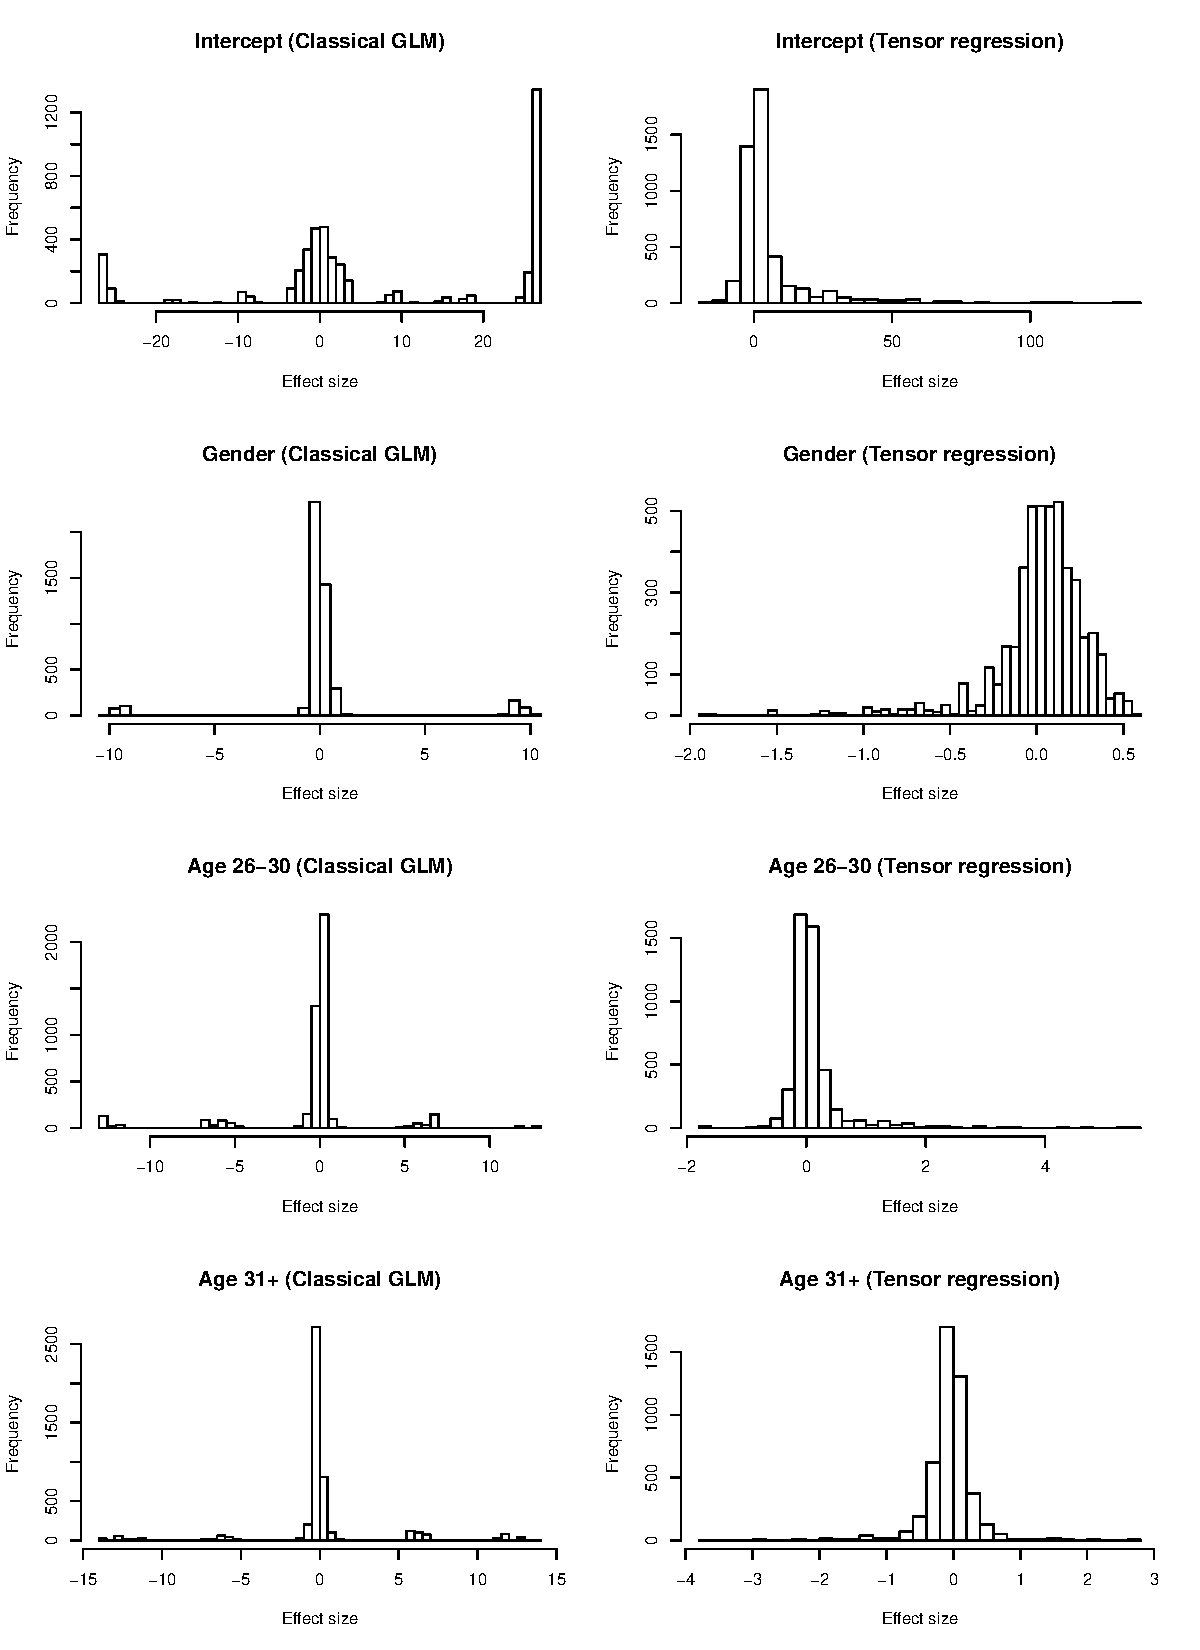
\includegraphics[width=17cm]{compare.pdf}

\bibliographystyle{unsrt}
\bibliography{tensor_wang}

\end{document}